\documentclass[conference]{IEEEtran}
\IEEEoverridecommandlockouts
% The preceding line is only needed to identify funding in the first footnote. If that is unneeded, please comment it out.
\usepackage{cite}
\usepackage{amsmath,amssymb,amsfonts}
\usepackage{cleveref}
\usepackage{algorithmic}
\usepackage{graphicx}
\usepackage{textcomp}
\usepackage{xcolor}
\def\BibTeX{{\rm B\kern-.05em{\sc i\kern-.025em b}\kern-.08em
    T\kern-.1667em\lower.7ex\hbox{E}\kern-.125emX}}

\def\proj{{\textbf{AILARON\ }}}
\def\proje{{\textbf{AILARON}}}
\newcommand{\cmt}[1]{{\color{red}{#1}}}

\begin{document}

% \title{Towards a system for Adaptive sampling of processes floating
%   with the current*\\
\title{Towards BioMapping: Autonomous Exploration for water column Biomass\\
% {\footnotesize \textsuperscript{*}Note: Working title}
%\thanks{Identify applicable funding agency here. If none, delete this.}
}

\author{\IEEEauthorblockN{
Andreas V{\aa}ge\IEEEauthorrefmark{1},
Tor Nordam\IEEEauthorrefmark{2},
Aya Saad\IEEEauthorrefmark{1},
Annette Stahl\IEEEauthorrefmark{1},
Martin Ludvigsen\IEEEauthorrefmark{3},
Kanna Rajan\IEEEauthorrefmark{4},
}
\IEEEauthorblockA{\IEEEauthorrefmark{1}
\textit{Dept. of Engineering Cybernetics},
\textit{Norwegian University of Science and Technology (NTNU)},
Trondheim, Norway \\
}
\IEEEauthorblockA{\IEEEauthorrefmark{2}
\textit{Dept. of Environment and New Resources},
\textit{SINTEF Ocean},
Trondheim, Norway \\
}
\IEEEauthorblockA{\IEEEauthorrefmark{3}
\textit{Dept. of Marine Technology},
\textit{NTNU},
Trondheim, Norway \\
}
\IEEEauthorblockA{\IEEEauthorrefmark{4}
\textit{Underwater Systems and Technology Laboratory},
\textit{ University of Porto},
Porto,  Portugal \\
}
}
\maketitle

% \begin{abstract}

% \end{abstract}

\begin{IEEEkeywords}
AUV, Machine Learning, Sampling, Gaussian Process, AI Planning, Plankton imaging
\end{IEEEkeywords}

\section{Introduction and Motivation}

Planktonic biomass forms the fundamental food source for consumers at
higher trophic levels. They play a significant role in producing more
than $50\%$ of the global oxygen supply. Hence, studying their
community structure, abundance, and dispersion across the ocean is a
primary research concern. To avoid transferring planktonic organisms
to the lab or applying ship-based point profiling as traditional
approaches suggest, we propose, an AUV control system with a framework
that images, identifies, and measures targeted plankton spatial spread
in-situ, akin to a ``sniffer dog''.  The software framework itself
identifies target taxa hotpots related to the upper water-column
microbial biology. Then, it adaptively plans the tracking of the
suggested hotspots for further exploration, allowing for accurate
modeling of targeted biological phenomena, which is an essential task
for marine biologists and the management of marine ecology.
%Big picture stuff..

\proj (\textbf{A}utonomous \textbf{I}maging and \textbf{L}earning
\textbf{A}i \textbf{RO}bot identifying pla\textbf{N}kton taxa in-situ)
for upper water-column microbial biology that images, processes,
analyzes, classifies plankton-based imagery in-situ in order to enable
intelligent onboard targeted sampling.

%\section{Motivation}

\section{Related Work}

Earlier work on robotic adaptive sampling in the upper water column
typically models the temporal property caused by the current as noise
under the assumption that the sample time-span is short enough
compared to the current velocity so that the transportation is
negligible or the current and the process being observed are in a
stationary equilibrium \cite{fossum18b}.  Incorporating the current into the model is
ambitious, but numerical ocean models provides more accurate forecasts
and small and improved acoustic sensors allows AUVs to directly
measure local current profiles.\cmt{give citations with a bibliography}.


% The following section describes one attempt to estimate and include
% the current into the models used for adaptive sampling; enabling the
% AUV to follow interesting processes along the current over time.

\section{Technical Description}

In \proj the process monitored are microbial biology and a novel
camera has been implemented into the hull of a AUV.  It continuously
captures images of particles floating trough its capture volume,
magnifying them while keeping them in focus over the entire capture
volume.  The raw images are processed and classified by a
state-of-the-art deep learning model on-board the AUV, resulting in a
stream of detected particle classes along with prediction confidences.
This stream is accumulated and interpreted as concentration
measurements of the different classes with accompanying measurement
variances.

For now we only consider one feature at a time, i.e. the total
concentration of particles, but extending the system to multiple
classes is possible.  Also other observable processes then microbial
biology could be monitored with the same system.

\subsection{Automated Planning and Execution}

The system is implemented as a set of sense, plan, act loops, communicating with each other trough goals and observations. \cite{rajan12}
The overall sense, plan and act loop for the \proj is seen in \cref{fig:sensePlanActLoop}. 
%(\cmt{This is abrupt. Most readers without an AI background won't know what the sense-plan-act loop is. Plus you should cite prior work there})
%\cmt{This a very different notion of SPA, but its good!}
\begin{figure}[tbp]
\centerline{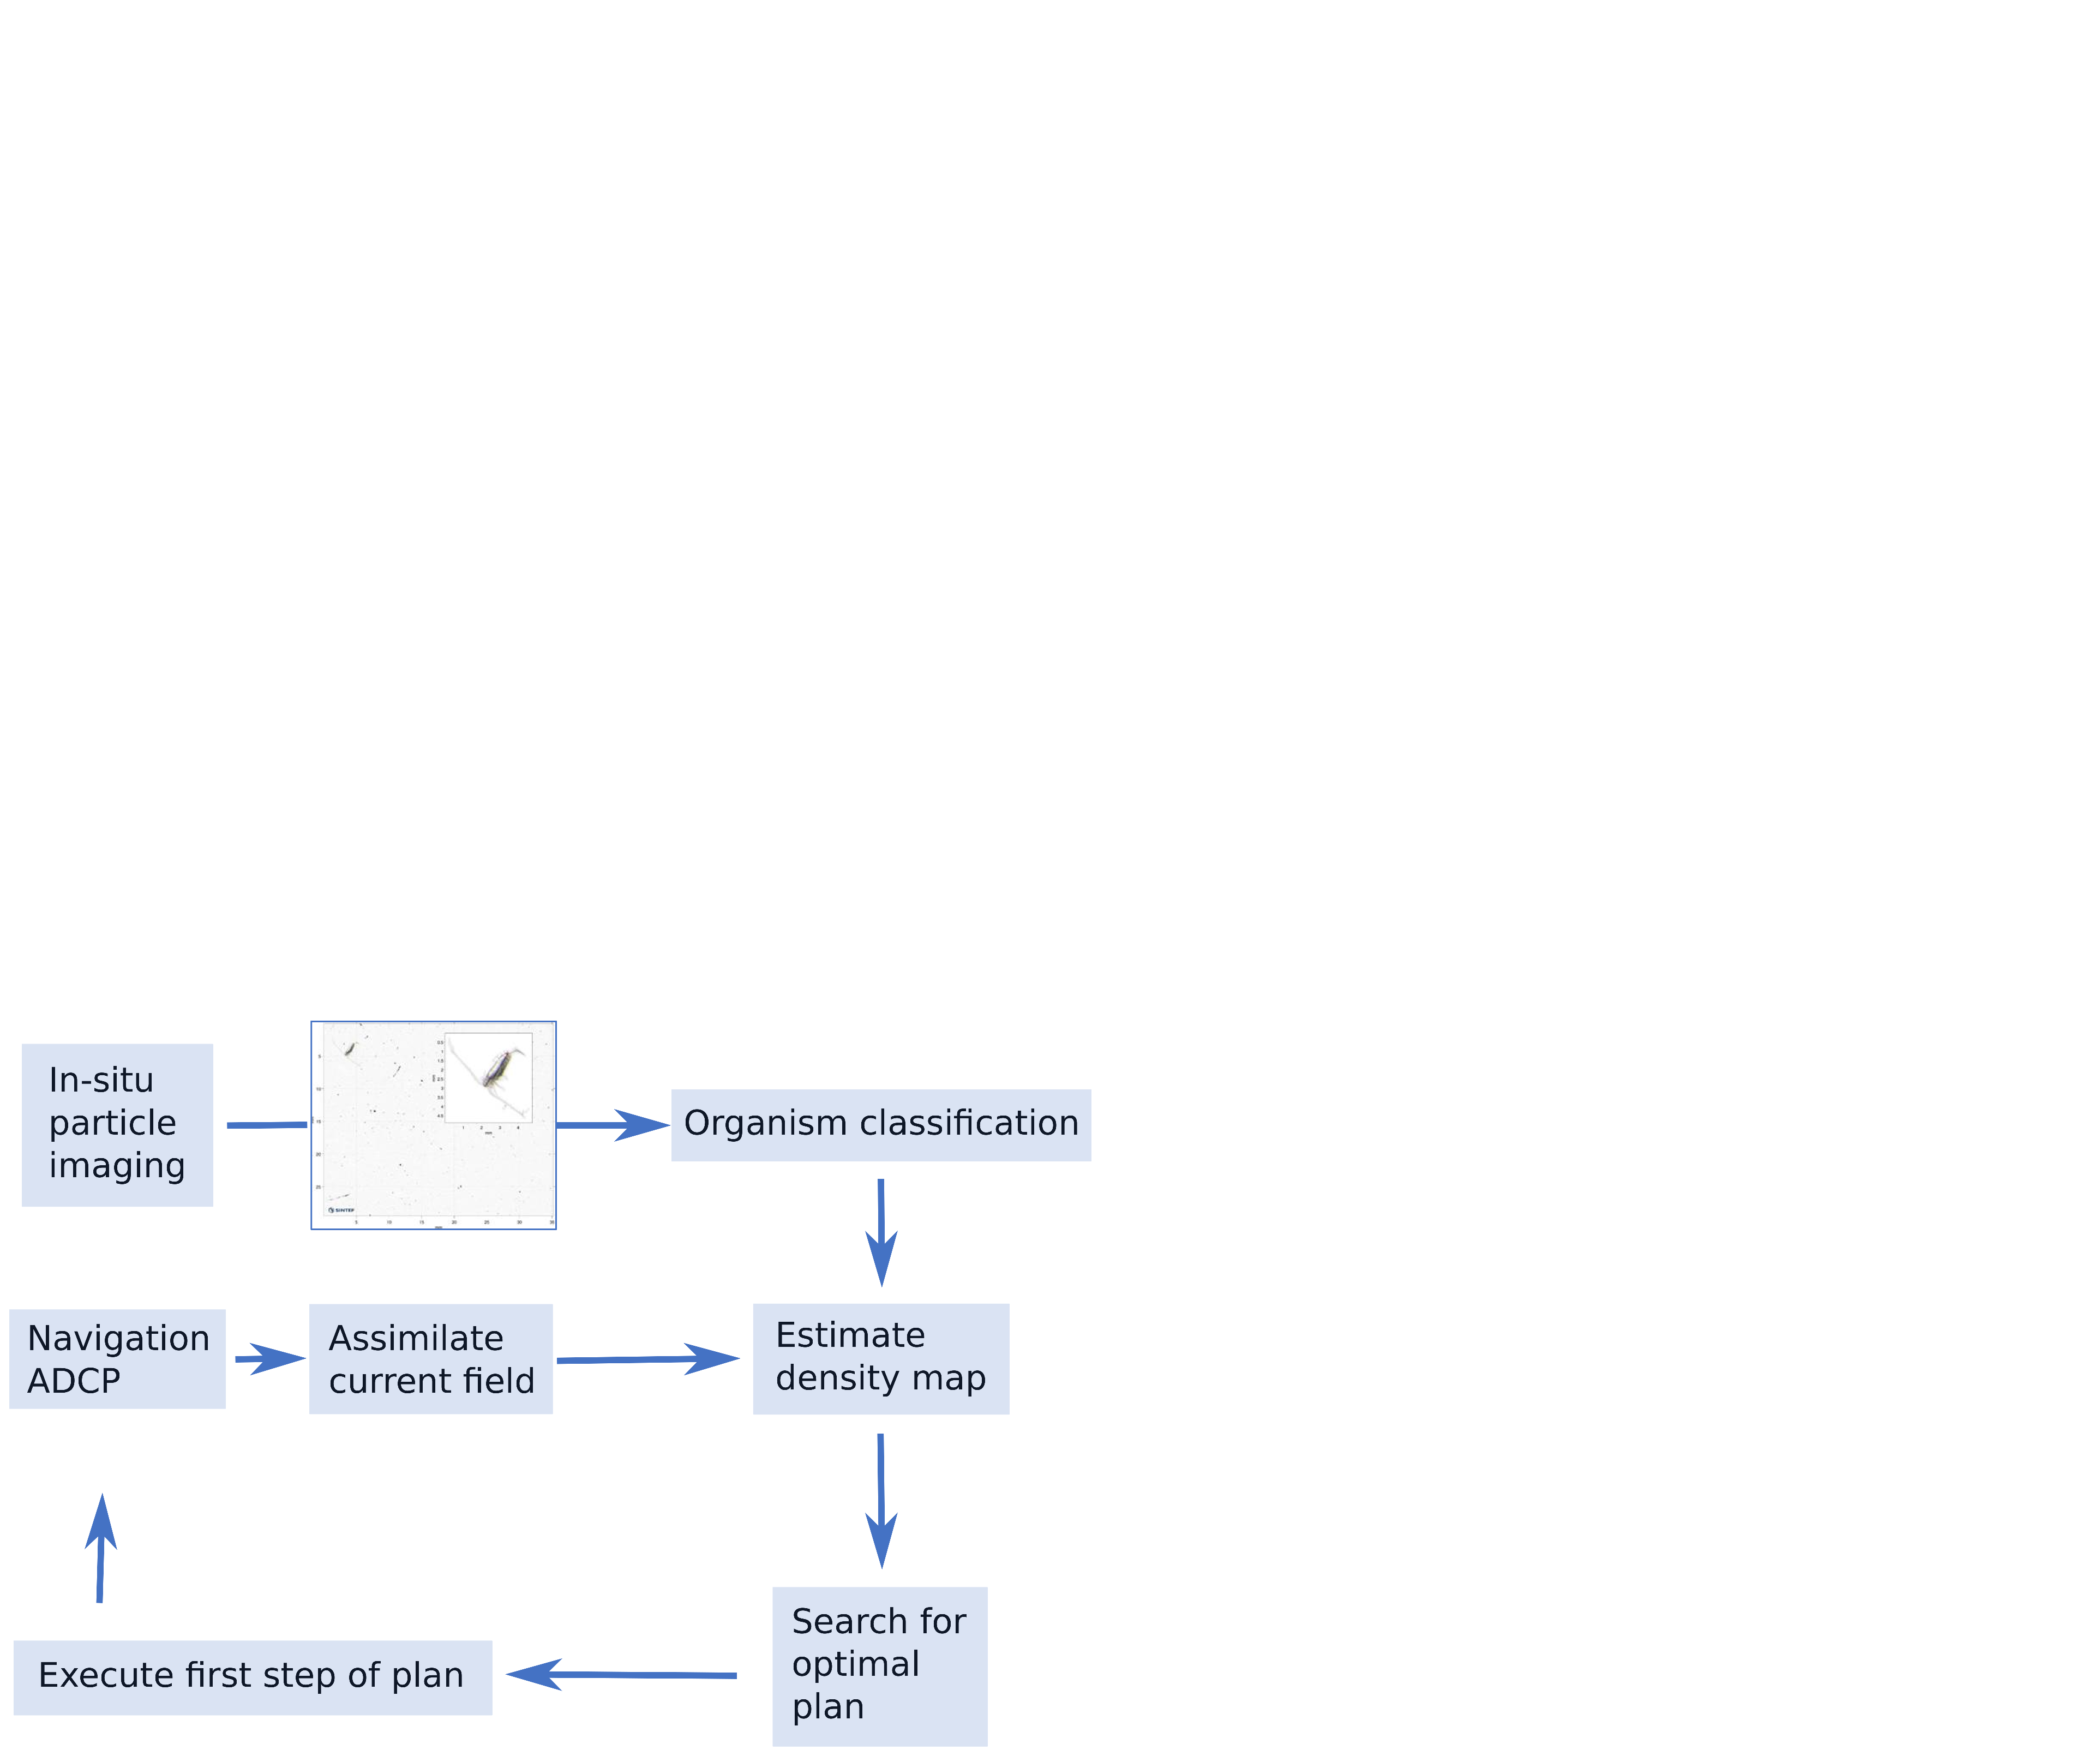
\includegraphics[width=0.9\linewidth]{figures/workflow-simplified.eps}}
\caption{The overall control loop running on board the AUV in \proje. After accumulating the measurements into the models, a plan for further data collection is found. The AUV will then start executing the plan, and thus gather new measurements, and will thus continuously update the plan.}
\label{fig:sensePlanActLoop}
\end{figure}
The executable plan consists of way-points for the low level control software to follow and commands for turning on and off scientific sensors, but also controls when new way-points need to be generated and the necessary steps to do so.

\subsection{Spatio-Temporal modelling}
As the spatial density of microbiology is not stationary, but changes over time we model it as spatio-temporal process. 
A local current model is used to predict the temporal movement of the process, by seeding an ensamble of particles over the model and transport each particle individually into the same temporal plane.
Once in the same temporal plane we consider it a standard spatial statistics problem and interpolate between the particles using Gaussian Process Regression/Kriging.

\paragraph{Local Current Model}
Represented as a 4D (space and time) vector field over the operational area of the AUV, it is either generated prior to missions based on the Numerical hydrodynamic model SINMOD \cite{slagstad2005} or accumulated during the mission from acoustic doppler current
profiler (ADCP) measurements on the AUV.

\paragraph{Particle Transport}
A Lagrangian particle transport model, derived from previous and ongoing
work at SINTEF \cite{Rye2006}, is run onboard the vehicle.
Particles are transported individually, using a variable-time step
integrator \cite{Dormand1980} through the current field, applying a random walk with the local diffusivity.

\paragraph{Gaussian Process Regression} 
Once the particles has been transported into the same temporal plane, Gaussian Process Regression is performed over the particles to estimate the spatial structure of the microbiology concentrations.
Gaussian process regression is data driven and requires very few parameters, which is important as the process observed is little known, making it hard to fit a parameter based model.
In addition to estimating the mean predicted values (the Kriging surface)
Gaussian Process regression also estimates the uncertainty, which is
later used to balance exploration vs exploitation when deliberating
where the AUV should go next.

%(\cmt{Cite. This is confusing; are you using a GP with the hydro-dynamic flow? I suspect what you want to say is, once a hot-spot has been identified, then to understand its spatial structure (size, extant and potentially as a result, the community (of the micro-organism) structure), one needs to do a GP (a la, work in Runde). Right?})
\subsection{Path Generation}

\paragraph{Objective Function}
The objective function is calculated over the estimated GP model along
the path candidate.  It is based on three interests:

\begin{itemize}

    \item scientific interest in particular plankton classes. 
    \item Exploitation: maximise expected measured concentration
      according to the kriging surface. 
    \item Exploration: minimise model variance by sampling from
      previously little visited areas. 

\end{itemize}

(\cmt{This is very abrupt. You want to say where the GP is being used,
  but after you talk about the plan-exec, since it is the plan-exec
  component which determines when to activate the GP and modify the
  kernel. There should be a nice flow between when you introduce the
  GP with the rest of the para's below. And after Plan/Exec.}).

\paragraph{Path Heuristics}

The goal is to find the path which maximises the objective function
based on the estimated GP model.  Only the first part of the path will
be traversed before new measurements are incorporated into the model
and a new path is deliberated, however the path should be longer than
the first step to achieve long term goals.  However allowing any kind
of path requires infinite evaluations of the objective function.  The
search is made more efficient by utilising traditional survey paths as
heuristics. E.g the standard square survey showed in
Fig.~\ref{fig:munkholmen} is parameterised by the covered rectangle
and its density, which is significantly fewer parameters to optimise
compared to specifying each line individually.
%Bresenham's line algorithm

All code is open source and based on open source projects. Including
the AUV control and navigation software (DUNE) and mission control
(Neptus)\cite{pinto2013lsts}.

\section{Experimental Results}

The system has been tested and verified in simulations and on historic
data. Fig.~\ref{fig:munkholmen} shows the planned path based on real
data from a survey in the Trondheim fjord in April 2020, during an
annual algae bloom. The planned path is maximising the expected
concentration of detected algae, while also minimising the variance of
the estimated Gaussian process.

\begin{figure}[tbp]
  \centering
  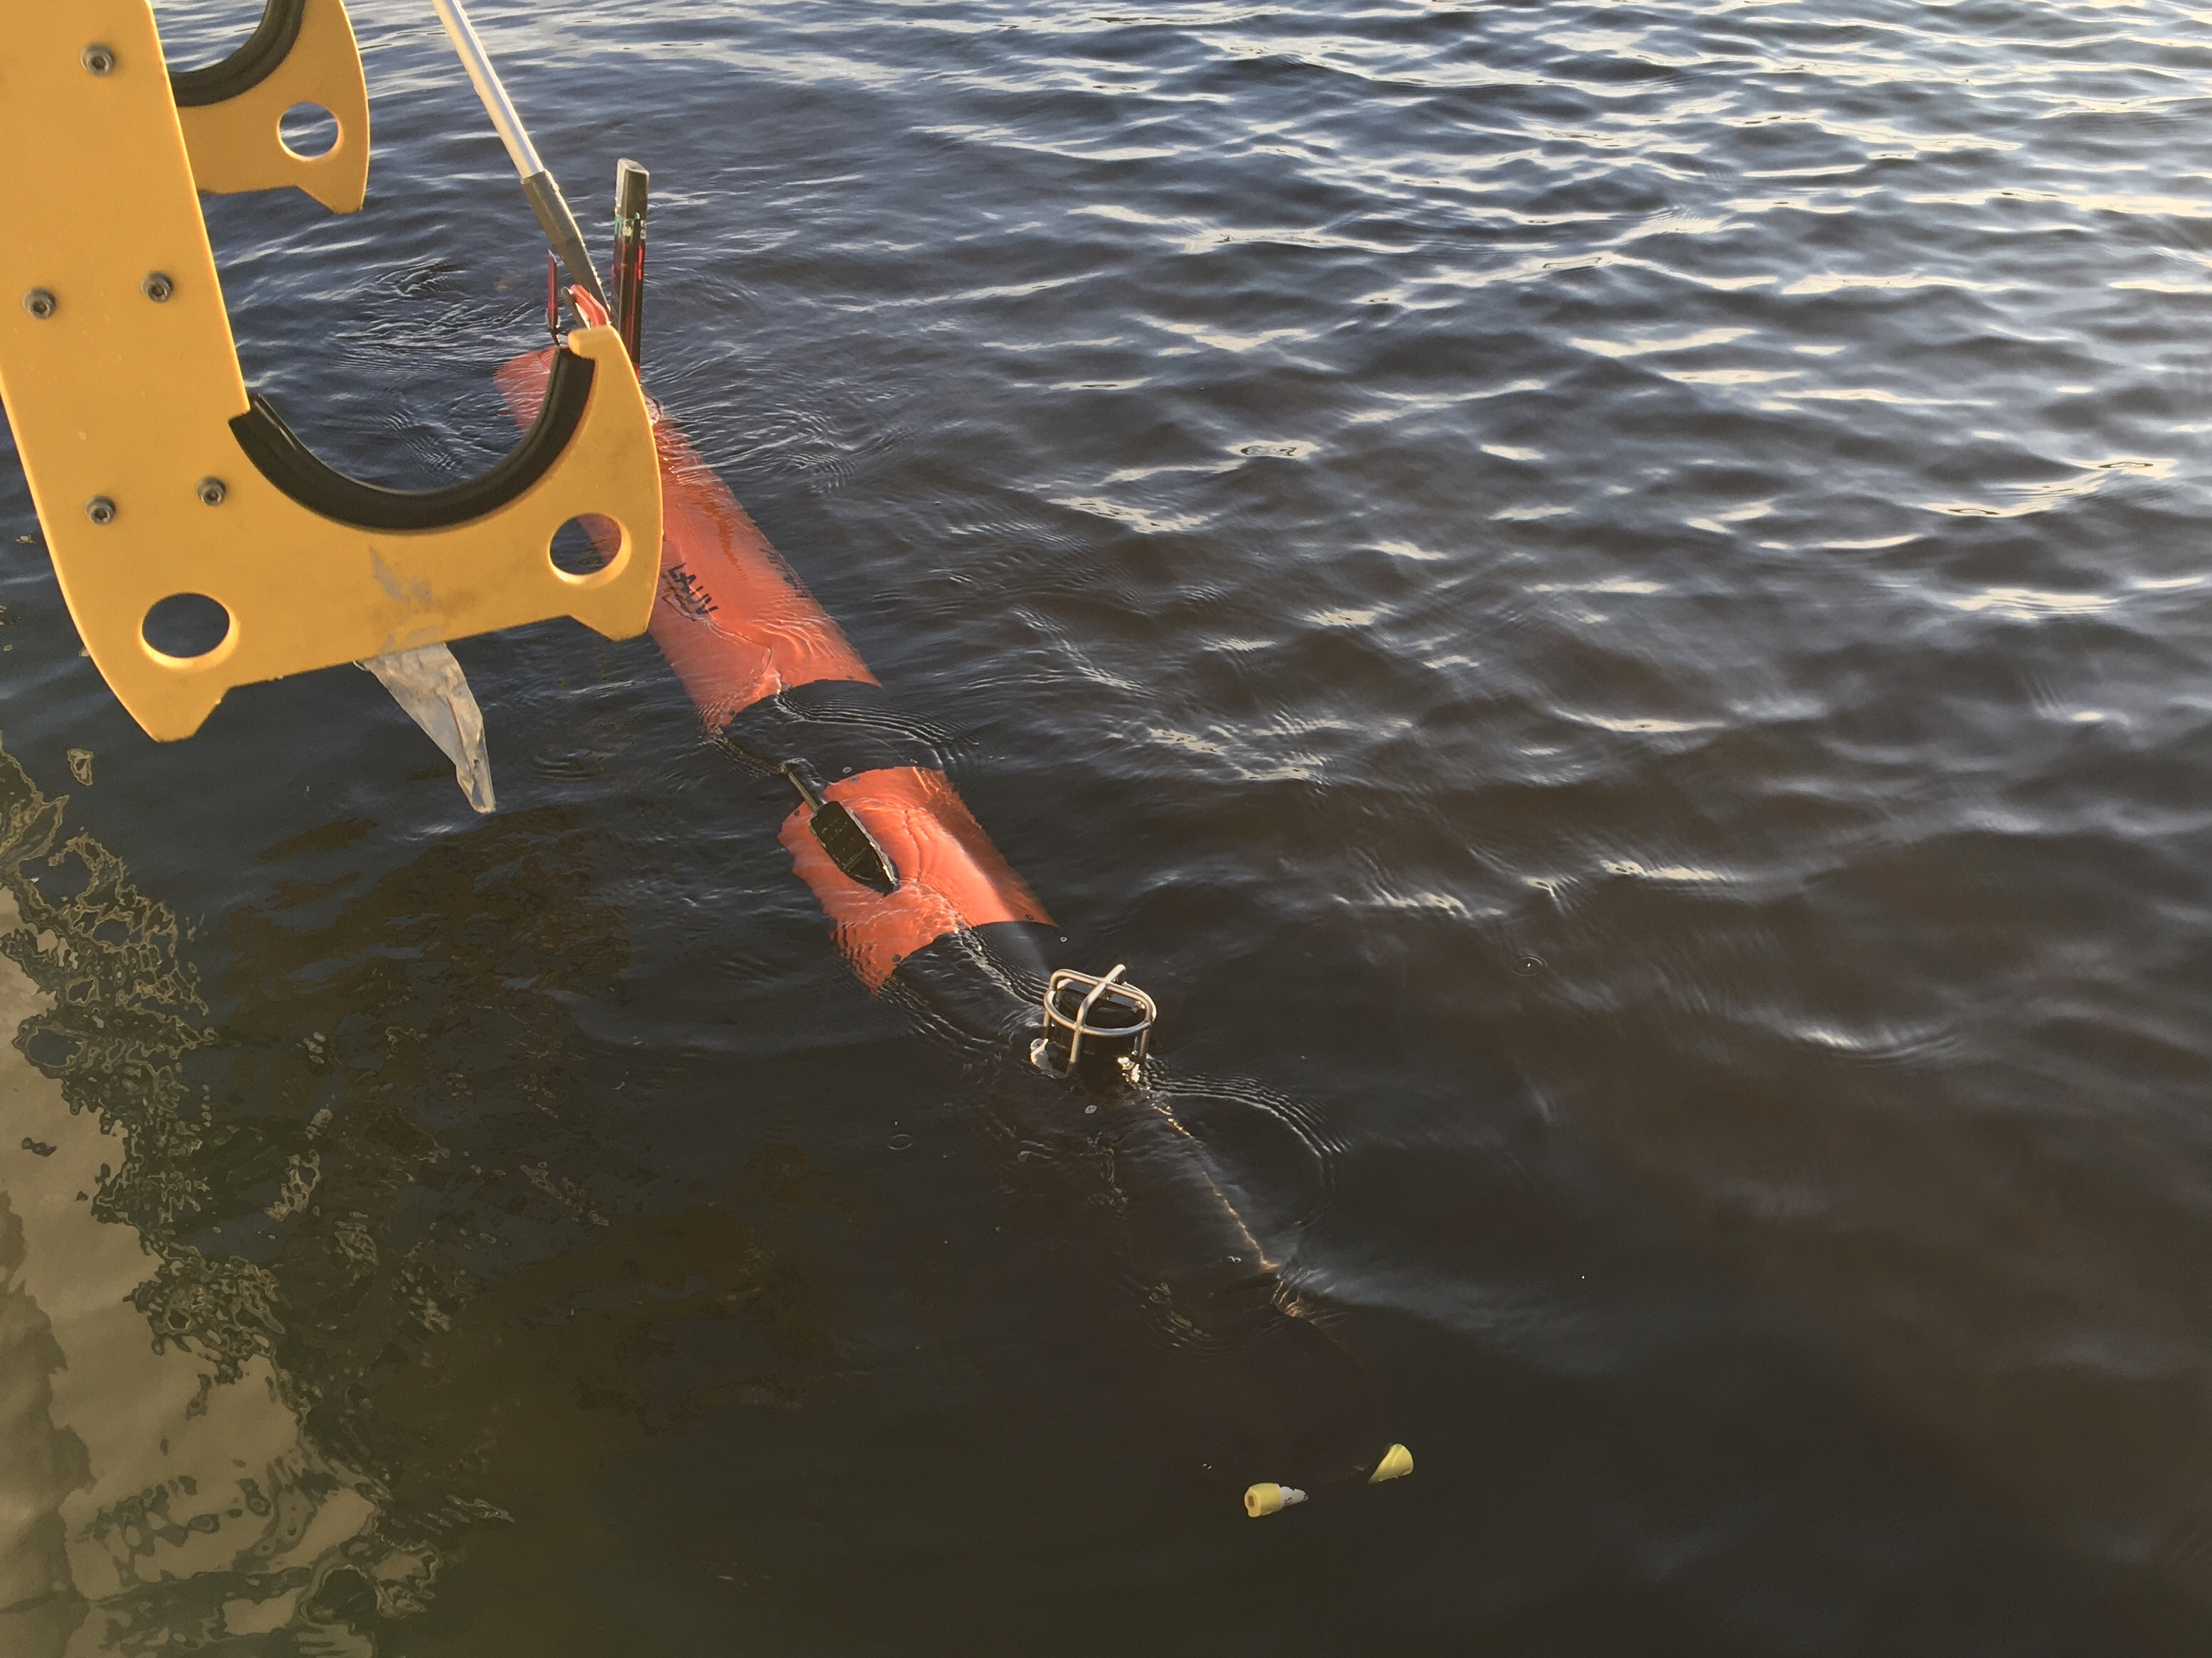
\includegraphics[width=\linewidth]{figures/Roald.jpeg}
  \caption{The Light Autonomous Underwater Vehicle (LAUV) Roald, used in
    \proje, being picked up at the end of a mission in the Trondheim
    fjord.}
  \label{fig:roald}
\end{figure}

\begin{figure}[tbp]
  \centering
  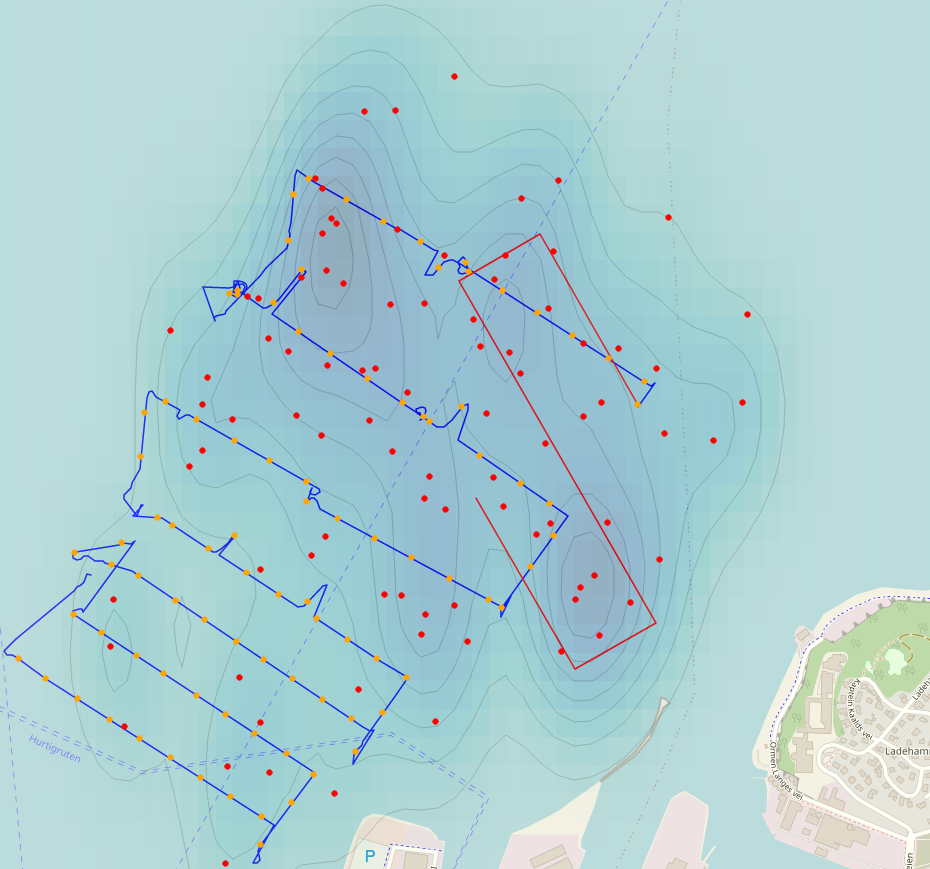
\includegraphics[width=\linewidth]{figures/munkholmen_planned_path.png}
  \caption{The AUV has traversed the blue path and gathered data (orange
    points), which has been transported with the current, and are now
    estimated to be located at the red points.  The contour shows the
    predicted concentration for which the red path is maximizing
    expected measured concentration and minimising model variance per travelled distance.}
  \label{fig:munkholmen}
\end{figure}

Future steps include experimentation with the AUV operating
autonomously in open waters.

% \section*{Acknowledgment}
% This work was supported by the Research Council of Norway through the FRINATEK/IKTPLUSS program, project number 262701.

\bibliographystyle{IEEEtran}
\bibliography{references}


\end{document}
